\documentclass{trlnotes}
\usepackage{trmath}
\addcompatiblelayout{commonplace}
\setlayout{commonplace}
\usepackage{trthm}
\usepackage{trsym} 
\usepackage{trphys}
\input{mdefs}
\usepackage{silence}
\usepackage{tikz}
\WarningFilter{latex}{Reference}
\graphicspath{{../../img/}}
\begin{document}

\paragraph{Устойчивость собственных чисел при возмущении матрицы}
\label{par:lin::eigenstab}

Пусть $A$~"--- линейный оператор $\R^s \to \R^s$, $x, b$~"--- векторы-столбцы в $\R^s$.
Здесь будет столько матриц и векторов, что рисовать шляпы не будем, и так понятно 
кто есть кто.

Какие задачи вообще можно здесь решать
\begin{enumerate}
  \item Решение линейной системы $Ax = b$
  \item Поиск собственных чисел $Ax = λx$
\end{enumerate}

Какие при этом могут возникнуть ошибки
\begin{enumerate}
  \item Ошибки округления (алгоритма)
  \item Ошибки начальных данных (неустранимые)
\end{enumerate}

Посмотрим, как оценить ошибки вычисления. 
Пусть $\circ$~--- какая-то операция, а $\circledcirc$~"---  её машинное представление.
Существуют два подхода
\begin{enumerate}
  \item \emph{Прямой анализ ошибок}\par
    Просто учитываем погрешность $a \circ b$ как ошибку округления. Часто
    делают так ($ε_M$~"--- <<машинный эпсилон>>):
    \[
      a \circledcirc b = a \circ b \, (1 + ε), \quad ε \leqslant ε_M
    \]
  \item \emph{Обратный анализ ошибок}(метод эквивалентных возмущений)\par
    Сводим все ошибки к возмущениям начальных данных:
    \[
      a \circledcirc b = \ov~a \circ \ov~b, \quad \ov~a = a + Δa, \; \ov~b = b + Δb.
    \]
    \begin{enumerate}
      \item оцениваем эквивалентные возмущения
      \item оцениваем влияние возмущений
    \end{enumerate}
    получается, что мы все ошибки записали в неустранимые погрешности начальных
    данных
\end{enumerate}

Первый метод частно выдает неправданно большие оценки погрешности,
так что займёмся в основном вторым.

Разберёмся с корректностью задач.
\clause{Решение ЛСУ} ${}$

\begin{defn}[мера обусловленности]\label{defn:lin::eigenstab::condnum}
  $μ = \norm{A}\, \norm{A^{\smash{-1}}}$
\end{defn}
Почему она так выглядит?
Посмотрим какие вообще есть способы оценки вырожденности $A$
\begin{enumerate}
  \item $\det A$. Почти не бывает равным 0. К тому же, перемешивает большие и маленькие 
    собственные числа.
  \item $\dfrac{\norm{Ax}}{\norm{x}}$. Здесь мы пытаемся смотреть на ЛЗ строчек матрицы.
    Но не очень понятно с чем сравнить, чтобы понять близость к ЛЗ. Может быть компоненты
    матрицы маленькие.
  \item $\dfrac{\max \frac{\norm {Ax}}{\norm {x}}}{\min \frac{\norm{Ax}}{\norm{x}}}$ уже выглядит
    разумно. Преобразуем, используя определение нормы (конечномерного) оператора
    \[
      \begin{aligned}
        \max \frac{\norm {Ax}}{\norm {x}} &= \norm{A} \\
        \min \frac{\norm {Ax}}{\norm {x}} &= \min \frac{\norm {y}}{\norm {A^{\smash{-1}}y}} = 
        \frac{1}{\frac{\norm{A^{\smash{-1}}y}}{\norm{y}}} = \norm{A^{{-1}}}^{-1}.
      \end{aligned}
    \]
    А это очень похоже на определение выше.
\end{enumerate}

\begin{lem}\label{lem:lin::eigenstab::idaddinv}
  $\norm{B} < 1\so \exists\,  (I-B)^{-1} \land \norm{(I-B)^{-1}}  \leqslant \dfrac{1}{1 -\norm{B}}$ 
\end{lem}
\begin{prf}
  Рассмотрим систему $x - Bx = y$. Будем искать решение методом простой итерации:
  $x_{n+1} = f(x_n) = B x_n + y$. Покажем, что он сходится. Для этого нужно убедиться что 
  $f$~"---  сжимающее отображение.
  \[
    \norm{f(x) - f(x')} = \norm{B(x-x')} \leqslant \norm{B} \norm{x-x'} < \norm{x-x'}
  \]
  Решение нашлось $\forall\, y \so \exists\, (I-B)^{-1}$.
  Теперь получим оценку нормы
  \[
    \forall\,x \holds x = Bx + y \so \norm{x} \leqslant \norm{B}\norm{x} + \norm{y} 
    \so \norm{x} \leqslant \dfrac{1}{1 -\norm{B}} \norm{y}
  \]
  Тогда это верно и для $\max \norm{x}/\norm{y} = \norm{(I-B)^{-1}}$
\end{prf}

Теперь, оценим, наконец, погрешность решения СЛУ.
\begin{thrm}\label{thrm:lin::eigenstab::stab}
  Рассмотрим возмущенную задачу: $\ov~Ax = \ov~b$.
  Введём относительную и абсолютную погрешность $A, x, b$:
  \[
    \begin{aligned}
      &ΔA = \ov~A - A, &  &Δx = x - x^*, & &Δb = \ov~b - b \\  
      &δ_A = \frac{\norm{ΔA}}{\norm{A}}, & 
      &δ_x = \frac{\norm{Δx}}{\norm{x*}}, &  
      &δ_b = \frac{\norm{Δb}}{\norm{b}} \\  
      x^* &\text{~--- невозмущенное решение} \span\omit\span
    \end{aligned}
  \]
  Тогда
  \[
    δ_x \leqslant \frac{μ(A)}{1-μ(A)δ_A}\, (δ_A + δ_b)
  \]
\end{thrm}
\begin{prf}
  Раз $x^*$~"--- решение $Ax^* = b$ 
  \[
    \begin{aligned}
      A'x = b' &\iff (A + ΔA) \, (x^* + Δx) = b + Δb \iff (A + ΔA)Δx  = -ΔA x^* + Δb \\
               &\iff \Bigl(I - (-A^{-1} ΔA)\Bigr) \,\frac{Δx}{x^*} = -A^{-1}ΔA +
                 A^{-1}\frac{Δb}{x^*}
    \end{aligned}
  \]
  Из леммы выше 
  \[
    \norm{\frac{Δx}{x^*}} \leqslant \frac{1}{1-\norm{A^{\smash{-1}}}\norm{ΔA}}\, 
    \left( \|A^{-1}\|\norm{ΔA} + \|A^{-1}\|\norm{\frac{Δb}{x^*}}\right)
  \]
  Из невозмущённой системы $\norm{x^*} \geqslant \|A\|^{-1}\norm{b}$, вспомнив определение 
  числа обусловленности осознаем $\|A^{-1}\|\norm{ΔA} = μ(A) \, δ_A$.
  Осталось переписать остальное через $δ$ и получить утверждение теоремы.
\end{prf}

\begin{rem}
  Из этой теоремы можно прикинуть ошибку решения ЛСУ. 
  Будем, как и обещали, использовать обратный анализ ошибок.
  Из-за неточного представления в памяти $δ_A, δ_b \sim ε_M$ (ну никак не меньше),
  так что $δ_x \sim C(s)\, μ(A)\, ε_M$‚ $C(s)$~"--- функция параметров задачи.
\end{rem}
\begin{rem}
  На оценку погрешности ещё влияют индивидуальные особенности методов.
  Например, в методе исключения Гаусса часто накапливается ошибка из-за
  деления на маленькие ведущие элементы.
\end{rem}

\clause{Поиск собственных чисел}${}$\\

Некий полезный набор фактов из линейной алгебры, который совсем не
стоит забывать
\begin{enumerate}
  \item $Au - λu$~"---  уравнение на собственные числа и собственные вектора.
  \item $p_A(t) = \det (A -tI)$~"--- характеристический многочлен.
  \item матрицы можно приводить к ЖНФ
  \item ЖНФ~"--- диагональ из жордановых клеток:
    \[
      J_p(a) = \begin{pmatrix}
        a & 1      & \\
          & \ddots & 1\\
          &        & a\\
      \end{pmatrix}\colon\;  p × p, \qquad p_{J_p(a)}(t) = (a-t)^p 
    \]
  \item алгебраическая кратность собственного числа~"--- кратность его как корня
    характеристического многочлена. Совпадает с размерностью корневого
    подпространства ($V(λ)$).
  \item геометрическая кратность~"--- размерность собственного подпространства
    $(V_λ)$.
  \item геометрическая кратность $\leqslant$ алгебраической, 
    ибо $\dim V_λ \leqslant V(λ)$.
  \item собственные числа самосопряженных операторов вещественные.
  \item из собственных векторов самосопряжённого оператора можно собрать ортогональный
    базис.
\end{enumerate}
\begin{prop}
  Для самосопряжённого положительно определённого оператора
  \[
    \max λ_A = \max \frac {(Au,u)}{(u,u)}, \quad \min λ_A = \min \frac {(Au,u)}{(u,u)}
  \]
\end{prop}
\begin{prf}
  Например, через теорему об условном экстремуме
\end{prf}
\begin{prop}
  $\norm2{A} = \sqrt{\max λ_{A^*A}}$
\end{prop}
\begin{prf}
  Эвклидова норма согласована со скалярным произведением, так что
  \[
    \max \frac{\norm2{Ax}}{\norm2{x}} = \max \frac{(Ax,Ax)}{(x,x)} = \max
    \frac{(A^*Ax,x)}{(x,x)}.
  \]
  А дальше можно глянуть утверждение выше.
\end{prf}
В принципе это сработает для любой нормы, согласованной со скалярным произведением.


Теперь наконец обсудим устойчивость
\begin{exmp}\label{exm:lin::eigenstab::unstab}
  Пусть \[
    A=J_p(a),\quad εB \that (εB)_{ij} = δ_{ip} δ_{j1}, \quad \ov~A = A+εB
  \]
  Оценим ошибку собственного числа 
  \[
    Ax + εBx = λx \iff \left\{\begin{aligned}
        ax_k + x_{k+1} &= λx_k, & k &\in 1\intrng p-1\\
        εx_1 + ax_p &= λx_p
    \end{aligned}\right.
    \so ε x_1 = (λ-a)^{p}x_1
  \]
  В итоге получается, что $λ = a + ε^{1/s}$\note{можно конечно корень из 1 в $\C$
  посчитать, но идея не изменится}

  Пусть $ε = 10^{-16}$ (удвоенная точность). Тогда уже на матрицах
  порядка $15$ ошибка $\sim 0.1$. Грустная оценка получилась.
\end{exmp}

\paragraph{Теорема Бауэра-Файка}
\label{par:lin::bf}

ситуация немного лучше, когда матрицы симметричные. Можно придумать
не такие грустные оценки, как в примере в предыдущем параграфе.

\begin{thrm}\label{thrm:lin::bf}
  Пусть $A$~"--- диагонализуемая матрица, $D^{-1}A D = Λ$. Тогда
  \[
    λ_{A+B} \text{~"--- с.ч. $A+B$}\so
    \exists\, λ_A\that\abs{λ_{A+B} - λ_A} \leqslant μ(D)\norm{B} 
  \]
\end{thrm}
\begin{prf}
  Построим отрицание 
  \[
    \forall\, λ_A\holds\abs{z - λ_A} > μ(D)\norm{B} \so 
    z \text{~"--- не с.ч. $A+B$}
  \]
  и будем его доказывать. Пусть $\abs{z-λ_A} > \norm{B}$. $\gprov$ $A+B-zI$~"--- неособая
  \[
    A - zI + B = D^{-1}\,(Λ-zI + DBD^{-1})\, D = D^{-1} \, (Λ-zI) \, 
    \bigl(I+\underbrace{(Λ-zI)^{-1} D BD^{-1}}_C\bigr)\, D
  \]
  $D$, $(Λ-zI)$ неособые по условию. Воспользуемся леммой об обратимости
  (\ref{lem:lin::eigenstab::idaddinv}). Для этого нужно $\norm{C} < 1$:
  \[
    \norm{C} \leqslant \norm{(Λ - zI)^{\smash{-1}}}
    \underbrace{\|D^{-1}\| \norm{B} \norm{D}}_{μ(D)\norm{B}}
  \]
  Из утверждения в предыдущем параграфе, и отрицания к предположению теоремы 
  \[
    \norm{(Λ - zI)^{\smash{-1}}} = \sqrt{\max_k \abs{λ_k - z}^{-2}} 
    = \sqrt{\frac1{\min_k \abs{λ_k - z}^2}}  < \frac{1}{μ(D)\norm{B}}
  \]
  Как видно, у нас как раз получилось что $\norm{C} < 1$. А тогда и матрица выше обратима.
\end{prf}

\begin{cor}\label{cor:lin::bf::sadj}
  Для самосопряженных матриц
  \[
    λ_{A+B} \text{~"--- с.ч. $A+B$}\so
    \exists\, λ_A\that\abs{λ_{A+B} - λ_A} \leqslant \norm{B} 
  \]
\end{cor}
\begin{prf}
  Для них просто $D$~"---  унитарная, $\norm{D} = \norm{D^{\smash{-1}}} = 1$.
\end{prf}

По сути мы сейчас доказали что собственные числа устойчивы к возмущениям матрицы.
А вот что там с собственными векторами?

\paragraph{Устойчивость собственных векторов при возмущении матрицы}
\label{par:lin::eivstab}

Сразу поясним, какие вообще возникнут проблемы
\begin{exmp}\label{exmp:lin::eivstab::rotnostab}
  Пусть $A_1,A_2$ имеют разные с.ч. и с.в, а
  \[
    C = \begin{cases}I + εA_1, & ε \geqslant 0 \\ I + εA_2, & ε<0 \end{cases}.
  \]
  Тогда, как видно
  \[
    λ_C = \begin{cases}1 + ε λ_1, & ε \geqslant 0 \\ 1 + ε λ_2, & ε<0 \end{cases}, \quad
    u_C = \begin{cases}u_1, & ε \geqslant 0 \\ u_2, & ε<0 \end{cases}
  \]
  и в $u$ никакого $ε$ нету. Направление у них изменяется скачком при проходе через 0.
  А вот с $λ$ всё хорошо.

\end{exmp}
Проблемы, как видно, возникают в окрестности кратных собственных чисел, снятие вырождения
радикально меняет собственные подпространства. Давайте не делать кратных собственных чисел.
Может быть так всё будет хорошо? 

\begin{prop}\label{prop:::peigstab}
  Пусть $(λ_i, u_i)$~"---  собственные числа и векторы $A$, $(μ_i, v_i)$~"--- $A^*$,
  все $λ_i$ разные. Короче говоря, $A$ диагонализуема, но может быть не самосопряжённой.
  Рассмотрим возмущенную задачу на собственные числа и векторы: 
  $(A + ΔA)\,x = (λ+Δλ)\,x$.

  Тогда в линейном приближении\note{а если нет, то надо думать}
  \begin{enumerate}\everymath{\displaystyle}
    \item[\bullet] $p_i = \frac{\norm{u_i}\norm{v_i}}{(u_i, v_i)}$
    \item $\norm{Δλ_i} \leqslant p_i \norm{ΔA}$
    \item $δ{u_i} \leqslant \sum_{k=1}^s \frac{p_k}{\abs{λ_i - λ_k}} \norm{ΔA}$
  \end{enumerate}
\end{prop}

\begin{prf} Пойдём по порядку. 
  \begin{enumerate}\everymath{\displaystyle}
    \item $λ_i = \ov-{μ_i}$
    \item $(u_i, v_k) = 0$ при $i\neq k$
      \[
        \begin{aligned}
          (Au_i, v_k) &= λ_i (u_i, v_k) \\
          (u_i, A^*v_k) &= \ov-{μ_k} (u_i, v_k) \\
        \end{aligned} \so (λ_i - \ov-{μ_k}) \, (u_i, v_k) = 0 \so (λ_i - λ_k) \, (u_i, v_k) = 0
      \]
    \item $(Ax,v_i) = \ov-{\mu_i} (x,v_i) = λ_i (x, v_i)$
    \item $Δ λ_i(u_i, v_i) = (ΔAu_i, v_i)$
      \[
        (\ov~A \ov~u_i,v_i) = (\ov~λ_i\ov~u_i, v_i)  
        \so (ΔAu_i,  v_i) + 
        (A \overbracket[0.5pt]{Δu_i, v_i) = Δ λ_i (u_i, v_i) + λ_i(Δu_i}^{=}, v_i)
      \]
      отсюда уже легко вывести первый пункт.
    \item $(Δu_i, v_k) = (1-δ_{ik}) \, \frac{(ΔA u_i, v_k)}{(λ_i, λ_k)}$, аналогично предыдущему 
      пункту. Здесь выбрали $(Δu_i, v_i) = 0$ пожертвовав нормированностью $v_i$. Всё равно 
      одна лишняя степень свободы была.
    \item $Δu_i = \sum_{k=1}^s γ_k u_k$ \note{$u_i$ образуют базис, раз матрица диагонализуема; 
      корневые подпространства совпадают с собственными}, $γ_k = \frac{(Δu_i, v_k)}{(u_k, v_k)}$
  \item $Δu_i = \sum_{k=1}^s \frac{(ΔA u_i, v_k)}{(λ_i - λ_k)}\, \frac{1}{(u_i, v_k)}$, 
    отсюда очевиден второй
  \end{enumerate}
\end{prf}

\paragraph{Степенной метод}
\label{par:lin::powermethod}

\begin{defn}[Степенной метод]\label{defn:lin::powermethod}
  Пусть $A$~"--- диагонализуемая матрица порядка $s$.
  Построим итерации такого сорта, $x_0$ выбирается случайно.
  \[
    \ov~x_{n+1} = Ax_n, \quad x_{n+1} = \frac{\ov~x_{n+1}}{\ov~x_{n+1}^1} \quad
    \text{ (делим на первую компоненту) }
  \]
  Будем брать $\ov~x_{n+1}^1$ как оценку наибольшего собственного числа $A$ 
\end{defn}

Мотивировка у такого определения понятная~"---  если $x_n$ разложить по собственным векторам
$A$, то через много шагов наибольшее собственное число забьет все остальные.
Однако, нужно аккуратно сформулировать условия сходимости.

\begin{prop}\label{prop:lin::powermethod::conv}
Пусть для собственных чисел $A$ выполнено условие:
\[
  \abs{λ_1} > \abs{λ_2} \geqslant \dotsb \geqslant \abs{λ_s}
\]
Тогда степенной метод сходится к $λ_1$
\end{prop}
\begin{prf}
  Из определения степенного метода
  \[
    x_n = \frac{\ov~x_n}{\ov~x_n^1} = \frac{A x_{n-1}}{\left\{ A x_{n-1} \right\}^1} 
    = \frac{\left(\ov~x_{n-1}^1\right)^{-1}\, A\ov~x_{n-1} }
    {\left(\ov~x_{n-1}^1\right)^{-1}\, \left\{ A \ov~x_{n-1} \right\}^1} 
    = \dotsb = \frac{A^n x_0}{\left\{A^n x_0\right\}^{1}}
  \]
  
  Разложим $x_0$ по собственным векторам $A$, тогда
  \[
    x_0 = \sum_{k=1}^s c_k u_k \so A^n x_0  = c_1 λ_1^n \, u_1 + \sum_{k=2}^s c_k λ^n_k\, u_k 
  \]

  Отсюда переходим к пределу
  \[
    \begin{aligned}
      x_n &=  \frac{A^n x_0}{\left\{A^n x_0\right\}^{1}} = 
      \frac{c_1 λ_1^n \, u_1 + \sum_{k=2}^s c_k λ^n_k\, u_k }{c_1 λ_1^n \, u_1^1 + \sum_{k=2}^s c_k λ^n_k\, u_k^1 } =
      \frac{\frac{u_1}{u_1^1} + \sum_{k=2}^s c'_k \left(\frac{λ_k}{λ_1}\right)^n\, u'_k }
      {1 + \sum_{k=2}^s c'_k \left(\frac{λ_k}{λ_1}\right)^n\, {u'_k}^1 }  \xto{n\to \infty} \frac{u_1}{u_1^1}\\
      \so \ov~x_{n+1}^1 &= \left\{Ax_n\right\}^1 \xto{n\to\infty}  \frac{\{λ_1 u_1\}^1}{u_1^1} = λ_1
    \end{aligned}
  \]
  Так сработает для комплексных $λ$, поскольку 
  \[
    \lim_{x\to \infty}\abs{\left(\frac{λ_k}{λ_1}\right)^n - 0 } = 
    \lim_{x\to ∞}\left( \frac{\abs{λ_k}}{\abs{λ_1}} \right)^n = 0
  \]
\end{prf}

Посмотрим, что будет если нарушить условия утверждения выше
\begin{exmp}
  $λ_1 = λ_2 = λ$: ну это одно и тоже число, так неинтересно
\end{exmp}
\begin{exmp}
  $λ_1 = -λ_2 = λ$
  \[
    \begin{aligned}
      x_{2n} &\to \tfrac{c_1u_1 + c_2u_2}{c_1u_1^1 + c_2 u_2^1}, &
      \ov~x_{2n+1}^1 &\to  λ\tfrac{c_1u^1_1 - c_2u^1_2}{c_1u_1^1 + c_2 u_2^1} \\
      x_{2n+1} &\to \tfrac{c_1u_1 - c_2u_2}{c_1u_1^1 - c_2 u_2^1}, &
      \ov~x_{2n+2}^1 &\to  λ\tfrac{c_1u^1_1 + c_2u^1_2}{c_1u_1^1 + c_2 u_2^1} \\
    \end{aligned}
  \]
  подпоследовательности сходятся к разным числам
\end{exmp}

\begin{exmp}
  $λ_1 = Re^{i θ}$, $λ_2 = Re^{-i θ}$, раз матрица вещественная $c_2 = \ov-{c_1}$, $u_2 =
  \ov-{u_1}$
  \[
    \begin{aligned}
      x_{n} &\to \tfrac{2\Re\left(c_1u_1e^{inθ}\right)}{2\Re\left(c_1u_1^1e^{inθ}\right)}, &
      \ov~x_{n+1}^1 &\to R \tfrac{\Re\left(c_1u_1^1e^{i(n+1)θ}\right)}{\Re\left(c_1u_1^1e^{inθ}\right)}\\
    \end{aligned}
  \]
  кажется это вообще никуда не сходится.
\end{exmp}

Для недиагонализуемых может сходиться, но медленно.
\plholdev{пример с матрицей-производной}

\begin{defn}[Степенной метод со сдвигом]\label{defn:lin::powermethod::powershifted}
  Рассмотрим в степенном методе матрицу $A-tI$ вместо $A$. При этом ищется наиболее удалённое
  по модулю от $t$ собственное число.
\end{defn}

\paragraph{Обратный степенной метод}
\label{par:lin::inversepowermethod}

\begin{defn}[Обратный степенной метод]\label{defn:lin::inversepowermethod}
  Пусть матрица $A$~"---  неособая. Будем применять степенной метод для $A^{-1}$.
  Решим, что то, что нашлось~"---  наименьшее по модулю собственное число.
\end{defn}

\begin{prop}
  Пусть для собственных чисел $A$ выполнено условие:
  \[
    \abs{λ_1} < \abs{λ_2} \leqslant \dotsb \leqslant \abs{λ_s}
  \]
  Тогда обратный степенной метод сходится к $λ_1^{-1}$
\end{prop}
\begin{prf}
  \[
    \begin{aligned}
      A^{-1}x = λ_*x &\iff λx = λ_*^{-1}x = A x \\
        \abs{λ_1} < \abs{λ_2} \leqslant \dotsb \leqslant \abs{λ_s} &\iff
      \abs{λ_1^{-1}} > \abs{λ_2^{-1}} \geqslant \dotsb \geqslant \abs{λ_s^{-1}} 
    \end{aligned}
  \]
\end{prf}

\begin{defn}[Обратный степенной метод со сдвигом]\label{defn:lin::powermethod::invpowershifted}
  Рассмотрим в обратном степенном методе матрицу $A-tI$ вместо $A$.
  Метод при этом будет искать ближайшее к $t$ собственное число
\end{defn}
В частности, можно взять грубую оценку с.ч. и уточнить её таким методом.


\begin{defn}[Обратный степенной метод с переменным
  сдвигом]\label{defn:lin::powermethod::invpowervarshifted}
  Возьмём обратный степенной метод и слегка изменим шаг итерации.
  Помимо махинаций с $\ov~x_{n+1}$,
  \[
    t_{n+1} = t_n + μ_n^{-1}, \qquad μ_n = \ov~x_{n+1}^1
  \]
  Метод при этом будет искать ближайшее к $t_0$ собственное число
\end{defn}
Доказывать что такой алгоритм сходится мы не будем.
Зато можно понять почему он так устроен.
Поскольку $\ov~x_{n+1}$~"--- текущее приближение собственного вектора
\[
  \ov~x_{n+1} = (A-tI)^{-1}x_n \iff (A-tI)\ov~x_{n+1} = x_n \iff \ov~x_{n+1} = (λ_A-t)^{-1}x_n
\]
На каждом шаге$x_n^1 = 1$, так что
\[
  μ = \ov~x_{n+1}^1 = (λ_A - t)^{-1} \iff λ_A = t + μ^{-1}
\]

\paragraph{Двумерные вращения}
\label{par:lin::rot}
Будем рассматривать матрицы самосопряженных операторов. 
На всякий случай, снова приведём набор полезных фактов из
линейной алгебры.
\begin{enumerate}
  \item Унитарные операторы~"--- такие, что сохраняют скалярное произведение:
    \[
      U \that (Ux, Uy) = (x, y)
    \]
  \item $U^*U = 1\so U^{-1} = U^*$
  \item Если $A$~--- самосопряженный, $\exists\, U \that A = U^{-1}ΛU$, $Λ$ тут диагональная.
  \item Произведение унитарных операторов~"---  унитарный оператор
\end{enumerate}

Вернёмся на вещественную прямую.
Матрицы операторов сменили названия
\[
  \begin{aligned}
    \text{унитарные}& &&\to& &\text{ортогональные} \\
    \text{эрмитовы}& &&\to& &\text{симметричные}
  \end{aligned}
\]
Все утверждения выше сохранились.
Запишем ещё пару специфических для $\R^n$ фактов 
\begin{enumerate}[resume]
  \item Существует базис, в котором матрица ортогонального оператора~"--- диагональ из
    блоков такого сорта:
    \begin{description}
      \item[тождество:] \fbox{$1$} 
      \item[отражение:] \fbox{$-1$} 
      \item[вращение:] \fbox{$
          \begin{smallmatrix}
            \cos φ & -\sin φ \\[0.5em]
            \sin φ & \phantom{-}\cos φ
        \end{smallmatrix}$}
    \end{description}
  \item Если вся ортогональная матрица единичная кроме одного
    блока, то
    она простое отражение/вращение.
\end{enumerate}

Простые вращения ещё называются двумерными вращениями.
Все потому, что блоки такого сорта соответствуют двумерным инвариантным подпространстрам.

Будем потихоньку приводить матрицу $A$ к (по возможности) диагональному виду.
Посмотрим, как выглядит один шаг такого приведения
\[
  A \to C = O^T A O, \quad \text{$O$~"--- ортогональная}
\]

Если выполнить все выкладки (для краткости переобозначив $\cos$, $\sin$ за
$c$, $s$), получится
явное выражение для компонент $C$
\begin{equation}\label{eq:lin::rot::step}
  C \that \qquad  
    \begin{aligned}
               c_{ij} &= a_{ij}, & i,j &\neq p,q \\
      c_{pj} = c_{jp} &= c\,a_{pj} + s \,a_{qj}, &\quad j &\neq p,q \\
      c_{qj} = c_{jq} &= -s\,a_{pj} + c \,a_{qj}, &\quad j &\neq p,q \\
               c_{pp} &= a_{pp}\, c^2 + 2\,a_{pq}\, cs + a_{qq}s^2 \\
      c_{pq} = c_{qp} &= (a_{qq} - a_{pp})\,cs + a_{pq}\,(c^2 - s^2) \\
               c_{qq} &= a_{qq}\, c^2 - 2\,a_{pq}\, cs + a_{pp}s^2 \\
  \end{aligned}
\end{equation}

Как можно избавиться от внедиагональных членов:
\begin{enumerate}
  \item $c_{p-1,q} = 0$: вращение Гивенса
\begin{equation*}
  \begin{split}
    c_{p-1,q} &= -s\,a_{p,p-1} + c\, a_{q,p-1},\\
    c &= \cos \varphi, s = \sin \varphi
  \end{split} \so 
  \cos φ = \frac{a_{p-1,p}}{\sqrt{a_{p-1,p}^2 + a_{p-1,q}^2}}; \quad
  \sin φ = \frac{a_{p-1,q}}{\sqrt{a_{p-1,p}^2 + a_{p-1,q}^2}}
\end{equation*}
  \item $c_{p,q} = 0$: вращение Якоби
\begin{equation*}
  \begin{split}
    c_{p,q} &= (a_{qq} - a_{pp})\,cs + a_{pq}\,(c^2 - s^2) \\
    c &= \cos \varphi, s = \sin \varphi
  \end{split} \so 
  \tan φ = \frac{2a_{pq}}{a_{qq}^2 - a_{pp}^2}
\end{equation*}
\end{enumerate}
\paragraph{Лемма о правиле знаков при исключении}
\label{par:lin::signrule}

Вспомним пару фактов из линейной алгебры:
\begin{defn}
  Пусть $B(x, y)$~"--- симметрическая билинейная функция. Тогда функция одного аргумента
  $B(x,x)$ называется квадратичной формой. 
\end{defn}
\begin{enumerate}
  \item $\forall\, B(x,x) \; \exists\, A\that (Ax,x) = B(x,x)$, $A$~"--- самосопряженный.
    Это означает, что можно записать матрицу квадратичной формы и она симметрична.
  \item \emph{Закон инерции}: если привести матрицу квадратичной формы к диагональному виду, то
    количество элементов одного знака не зависит от способа приведения.
\end{enumerate}

Теперь можно сформулировать лемму.
\begin{lem}\label{lem:lin::signrule}
  Пусть $A$~"--- симметричная матрица.  Тогда число ведущих элементов одного
  знака в методе исключения Гаусса для такой матрицы совпадает с числом
  собственных чисел того же знака.
\end{lem}

\begin{prf}
  Рассотрим квадратичную форму $(Ax,x)$. Напишем её в координатах:
  \[
    (Ax,x) = \sum_{ij} a_{ij} x_i x_j = a_{11}x_1^2 + 2\sum_{i} a_{1j}x_1x_j + 
    \sum_{i,j \geqslant 2} a_{ij}x_i.
    x_j
  \]
  Будем приводить её к сумме квадратов стандартным способом (Лежандра).
  \[
    (Ax,x) = a_{11}^{-1} \,\biggl( \underbrace{\sum_{j}a_{1j}x_j}_{ξ_1^2}\biggr)^2
    + \sum_{i,j \geqslant 2} \Bigl(
      \underbrace{a_{ij} - \tfrac{a_{1i}a_{1j}}{a_{11}}}_{a'_{ij}}
    \Bigr)\,x_ix_j
  \]
  Внимательно присмотримся к $a_{ij}'$. Мы вычитаем из элемента строки такой же
  элемент первой строки, поделённый на первый элемент первой строки, умноженный
  на первый элемент данной строки. А это как раз шаг метода исключения Гаусса.

  Теперь приведём $A$ к ЖНФ. Поскольку она симметричная, $J_A$ диагональная. 
  На диагонали стоят собственные числа. 
  Сравнивая их c $a_{jj}$ и припоминая закон инерции, приходим к утверждению
  леммы.
\end{prf}

\paragraph{Метод Гивенса}
\label{par:lin:givens}

Вспомним, как выглядело вращение Гивенса

\begin{equation*}
  \begin{split}
    c_{p-1,q} &= -s\,a_{p,p-1} + c\, a_{q,p-1} = 0,\\
    c &= \cos \varphi, s = \sin \varphi
  \end{split} \so 
  \cos φ = \frac{a_{p-1,p}}{\sqrt{a_{p-1,p}^2 + a_{p-1,q}^2}}; \quad
  \sin φ = \frac{a_{p-1,q}}{\sqrt{a_{p-1,p}^2 + a_{p-1,q}^2}}
\end{equation*}
Будем строить повороты с $(p,q)$ в таком порядке, как на картинке ниже
\begin{center}
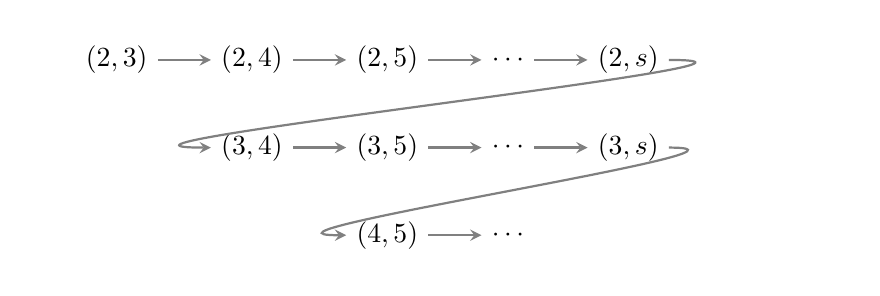
\begin{tikzpicture}[>=stealth, 
  thick, black!50, text=black]
  \matrix[row sep = 15, column sep = 20]{
    \node(b1) {$(2,3)$};&\node(p11){$(2,4)$};& \node(p12) {$(2,5)$};&\node(m1) {$\cdots$};&
    \node(e1) {$(2,s)$};\\
                        &\node(b2) {$(3,4)$};&\node(p21) {$(3,5)$};&\node(m2) {$\cdots$};&
    \node(e2) {$(3,s)$};\\
                        &                    &\node(b3) {$(4,5)$}; &\node(m3) {$\cdots$};\\
  };
  \path[->] 
    (b1)  edge (p11)
    (p11) edge (p12)
    (p12) edge (m1)
    (m1)  edge (e1)
    (e1)  edge [out=0, in=180] (b2)
    (b2)  edge (p21)
    (p21) edge (m2)
    (m2)  edge (e2)
    (e2)  edge [out=0,in=180] (b3)
    (b3)  edge (m3)
    ;
\end{tikzpicture}
\end{center}

На каждом шаге метода столбцы/строки с индексами $p$ и $q$ заменяются их линейными комбинациями.
При этом явно зануляется $(p-1,q)$ элемент.
А после предыдущих шагов $\forall j>1$ $(p-j, q)$, $(p-j, p)$ уже нули. 
Либо $p=2$ и выше просто ничего нет. Так что и
линейные комбинации <<верхушек>> столбцов будут нулями, 
и ничего испортиться не сможет. Про область нулей под диагональю можно особо
не думать, она получится автоматически, так как матрица симметричная на каждом
шаге.

После вращений Гивенса матрица стала трёхдиагональной.
\[
  (A - t I) = \begin{pmatrix}
    a_1 - t & b_1     & \\
    b_1     & a_2 - t & \ddots &\\
            &         & \ddots &b_{s-1}\\
            &         & b_{s-1}&a_s - t\\
  \end{pmatrix} 
\]
Введём $p_k$~--- угловые миноры.
порядка $k$ Из формулы разложения определителя по строке получаются рекуррентные
формулы для $p$
\[
  \begin{aligned}
    p_1(t) &= a_1 - t \\
    p_2(t) &= (a_2 - t) p_1(t) - b_1^2 \\
    p_k(t) &= (a_k - t) p_{k-1}(t) - b_{k-1}^2 p_{k-2}(t) \\
  \end{aligned}
\]
Как нетрудно заметить, последовательность $p_k(t)$ для 
фиксированного $t$~"--- это тоже самое что и $a_{kk}$ в лемме в предыдущем
параграфе (\ref{lem:lin::signrule}). Ну ведь правда, после
$k$ шагов метода Гаусса на диагонали вплоть до $k$ строки стоят $1$.
Так что угловой минор просто равен $a_{kk}$. 

Разберёмся теперь как искать собственные числа.
\begin{enumerate}
  \item Как корни характеристического многочлена, $χ(t) = p_s(t)$
  \item Методом бисекции\par
  Про этот пункт придётся написать чуть подробнее. Выберем какие-то 2 начальныx
  приближения $λ$, чтобы искать его между ними. Будем считать число перемен
  знака в последовательности $a_{kk}$.
  Нам нужно добиться чтобы перемена знака была всегда одна. Обычным методом
  половинного деления как раз можно к этому прийти.
\end{enumerate}


\paragraph{Метод Якоби}
\label{par:lin::jacobi}

Вспомним, как выглядело вращение Якоби
\begin{equation*}
  \begin{split}
    c_{p,q} &= (a_{qq} - a_{pp})\,cs + a_{pq}\,(c^2 - s^2) \\
    c &= \cos \varphi, s = \sin \varphi
  \end{split} \so 
  \tan φ = \frac{2a_{pq}}{a_{qq}^2 - a_{pp}^2}
\end{equation*}

Будем пытаться прийти к почти диагональной матрицей. Для этого надо
как-то измерять <<недиагональность>>.
Введём набор величин
\begin{itemize}
  \item $N^2(A) = \sum_{i,k} a_{ik}^{2} = \Tr (A^2)$
  \item $d^2(A) = \sum_{i,k} a_{ii}^{2}$
  \item $t^2(A) = \sum_{i\neq k} a_{ik}^{2} = N^2(A) - d^2(A)$
\end{itemize}

\begin{prop}\label{prop:lin::jacobi::nondiagest}
  После одного двумерного вращения ($C = O_{pq}^{T}AO_{pq}$)
  \[
    t^2(C) = t^2(A) - 2 a_{p,q} + 2 c_{p,q}^2
  \]
\end{prop}
\begin{prf}Пойдем по порядку
  \begin{enumerate}
    \item $N^2(C) = N^2(A)$, поскольку $C^2 = O^TAO\,O^TAO = O^{T}AO$, а след 
      подобных матриц совпадает.
    \item $t^2(C) = N^2(C) - d^2(C) = t^2(A) + d^2(A) - d^2(C)$
    \item $d^2(A) - d^2(C) = a_{p,p}^2 + a_{q,q}^2 - c_{p,p}^2 - c_{q,q}^2$, просто
      все остальные элементы на диагонали не поменялись.
    \item $a_{p,p}^2 + a_{q,q}^2 + 2a_{p,q}^2 = c_{p,p}^2 + c_{q,q}^2 + 2c_{p,q}^2$.

      Это можно либо явно проверить из формулы~\eqref{eq:lin::rot::step}, либо
      вспомнить что вращения квадраты норм матриц не изменяют, а эти 4 элемента
      преобразуются независимо от других. Разве что мы норму оператора не так 
      определяли.
  \end{enumerate}
\end{prf}
Метод Якоби как раз зануляет $c_{pq}^2$ на шаге, оптимально уменьшая таким образом
$t^2$.
Разберёмся как выбирать здесь $p$ и $q$. 

\begin{enumerate}
  \item Классический метод Якоби: 
    $p,q\that \abs{a_{p,q}} = \max\limits_{i\neq k}\abs{a_{i,k}}$.
    
    Оценим, как быстро он сходится
    \[
      a_{p,q}^2\, \tfrac{s\,(s-1)}2 \geqslant \sum_{i,k} a_{i,k}^2 \so
      t^2(C) \leqslant \left(1 - \tfrac{2}{s(s-1)}\right)\, t^2(A) 
    \]
    Неплохо, но поиск максимума $\sim O(s^2)$, а сам метод
    Якоби $\sim O(s)$. Подумаем как можно улучшить.
  \item Циклический метод Якоби: просто проходим по всем наддиагональным
    элементам много раз. 
  \item Циклический метод Якоби c барьером: выбираем $ε_i > 0$ и зануляем всё
    что больше него. Потом выбираем $ε_{i+1} < ε_{i}$ и повторяем.
\end{enumerate}

Разберёмся, как искать собственные числа и собственные векторы.
\begin{enumerate}
  \item С $λ$ всё просто~"---  они на диагонали матрицы. Корректность следует
    из теоремы Бауэра-Файка (\ref{thrm:lin::bf}), просто вычтем внедиагональные
    члены
  \item в качестве собственных векторов можно просто взять строки матрицы
    произведения всех двумерных вращений.
    
    Это сработает, поскольку собственные векторы диагональной
    формы~"--- $e_k$,
    \[
      λ_k e_k = Λ e_k = OA O^{T} e_k \iff A\,O^{T}e_k = λ_k O^{T}e_k,
    \]
    а $O^Te_k$ как раз $k$-ая строчка $O$.
\end{enumerate}

\paragraph{Две леммы о факторизации матрицы}
\label{par:lin::factor}

\begin{lem}\label{lem:lin::factor::lr}
  Пусть $A$~"--- неособая матрица с ненулевыми диагональными минорами
  Тогда
  \[
    \exists!\, L,R \that A = LR, \quad
    L = \begin{pmatrix}
      1 &  & \\
      \bullet  & \ddots  & \\
      \bullet &\bullet &1\\
    \end{pmatrix} , \qquad
    R = \begin{pmatrix}
      \bullet & \bullet & \bullet\\
        & \ddots  & \bullet\\
        &         &\bullet\\
    \end{pmatrix}.
  \]
  То есть раскладывается на произведение верхней/нижней треугольной.
\end{lem}
\begin{prf}
  Эта теорема~"--- матричная запись метода Гаусса. 
  Запишем явное выражение для первого шага
  \[
    a_{ij} = a_{ij} - \frac{a_{i1}a_{1j}}{a_{11}}, \quad i = 2, \dotsc, s
  \]
  Посмотрим на эту формулу как на преобразование $j$го столбца. Тогда матрица 
  такого преобразования имеет вид
  \[
    \begin{pmatrix}
      1 &   & & & \\
      \bullet  & 1 & & \\
      \vdots  & 0 & 1& \\
      \bullet  & 0 & 0& 1\\
    \end{pmatrix}
  \]
  понятно, что в случае $k$-го шага будет просто $k$-й столбик.
  Если мы будем перемножать такие столбики, они просто будут пристраваться рядом.
  Ну в самом деле, умножим нижнетреугольную  матрицу на такой столбик.
  $c_{ij} = \sum_{p}a_{ip}b_{pj}$, а при всех $j \neq k$ вместо $b_{pj}$ просто
  такой же член от единичной матрицы. А сохранение треугольности следует из
  треугольности $a_{ip}$.
  
  Чтобы убедиться в единственности, можно рассмотреть матричное равенство
  построчно. А у последовательного 
  набора этих равенств получается всего одно решение.
\end{prf}


\begin{lem}\label{lem:lin::factor::qr}
  Пусть $A$~"--- неособая матрица.
  Тогда
  \[
    \exists\, Q,R \that A = QR
  \]
  Здесь $R$ как в лемме выше, а $Q$~--- ортогональная.
\end{lem}
\begin{prf}
  Прогоним процесс ортогонализации Грамма-Шмидта для строчек $A$, 
  строчки $Q$ это полученный ортогональный базис. 
  При этом $Q = LA$, только на диагонали не обязательно $1$.
  А $L^{-1}$ уже будет верхнетреугольной.
\end{prf}

\paragraph{Теорема о сходимости итерированных подпространств}
\label{par:lin::iterspaceconv}

Вспомним про степенной метод из \ref{par:lin::powermethod}.
У него был недостаток, он не умел искать больше одного собственного числа.
Но мы и итерировали всего один вектор. Давайте обобщим.

\begin{defn}\label{defn:lin::iterspaceconv::iterbas}
  Пусть $A$~"--- диагонализуемая неособая матрица, 
  $\{x_{j}\}$~"---  базис в $\R^s$, 
  \begin{enumerate}
    \item $\bigl\{x_{j}^{(n)}\bigr\}=\bigl\{A^nu_j\bigr\}$~"--- 
      $n$-ный итерированный базис
    \item $L_s^{(n)} = \left\langle A^n x_1,\dotsc,A^n x_s\right\rangle$~"--- 
      $n$-ное итерированое подпространство.
  \end{enumerate}
\end{defn}
\begin{rem}
  Можно итерировать не весь базис, а, например, только $k$ векторов из $s$.
  Помимо добавления эпитетов, характеризующих размерность, 
  вводят $U_k=\left\langle u_1, \dotsc, u_k\right\rangle$~"---  $k$-мерное
  старшее собственное подпространство, а $\{u_j\}$~"--- базис из собственных
  векторов $A$.
\end{rem}

\begin{defn}\label{defn:lin::iterspaceconv::iterspconv}
  Говорят, что $P^{(n)} \to P$, если в $P^{(n)}$ существует базис, сходящийся к
  базису $P$.
\end{defn}

\begin{thrm}\label{thrm:lin::iterspaceconv::conv}
  Пусть $A$~"--- диагонализуемая неособая матрица, 
  \[
    \abs{λ_1} > \abs{λ_2} > \cdots > \abs{λ_s} > 0 \qquad\text{(все разные)}
  \]
  Тогда $L_k^{(n)} \to U_k$.
\end{thrm}
\begin{prf}
  Соорудим базис в $L_k^{(n)}$ который будем сходится к базису $U_k$.
  Пусть ${x_j}^k$~"---  исходный базис,\note{этого условия у нас не было, но
  без него не доказать невырожденность $\ov~C$.}
  \[
    \langle x_1, \dotsc, x_k \rangle \supset \langle u_1, \dotsc, u_k \rangle.
  \]
  Разложим его по $u_j$ и посмотрим на итерированный
  \[
    x^{(n)}_i = \sum_{\ell=1}^k c_{i\ell} \, λ_\ell^n u_\ell 
    + \sum_{\ell=k+1}^s c_{i\ell} \,λ_\ell^n u_\ell
  \]
  Домножим обе части на $D = \left(\ov~C\right)^{-1}$, $\ov~C$~"--- квадратный
  кусок $C$ размерами $k \times k$ из перых коэффициентов.

Рассмотрим $\ov~Z_{m}^{(n)} = \sum_{i=1}^k d_{m,i}\,x_{i}^{(n)}$, они явно базис $L_k^{(n)}$
в силу невырожденности $D$.
\[
\ov~Z^{(n)}_{m} = 
\sum_{\ell,i=1}^k \underbrace{d_{m,i}\,c_{i,\ell}}_{δ_{m\ell}} \,λ_{\ell}^n u_{\ell} + 
  \sum_{\ell=k+1,i=1}^{s,k} d_{m,i}\,c_{i,\ell} \,λ_{\ell}^n u_{\ell}
\]
Теперь поделим: $Z_{m}^{(n)} = \ov~Z_{m}^n \, λ_{m}^{-n}$, они всё ещё базис
$L_k^{(n)}$.
\[
  Z_{m}^{(n)} = u_{m} + \sum_{\ell \geqslant k+1,i} d_{m,i}\,c_{i,\ell} 
  \,\left(\frac{λ_{\ell}}{λ_m}\right)^n u_{\ell} \to u_m
\]
\end{prf}

\begin{defn}[Ступенчатый базис]\label{defn:lin::iterspaceconv::stairbasis}
  \begin{align}
    e_1 &= (1, x_{12}, \dotsc ) \\
    e_k &= (0, \dotsc, 0,  1, x_{k,k+1}, \dotsc ) \\
  \end{align}
\end{defn}

\begin{prop}
  Обычно базис пространства приводится к ступенчатому.
\end{prop}
\begin{prf}
  метод Гаусса
\end{prf}

можно ещё рассматривать, например, $e_1, \dotsc, e_k$ как базис $L_k$, нам
ведь неважно что там в следущих компонентах происходит.

\begin{thrm}\label{thrm:lin::iterspaceconv::stairbasis}
  Cтупенчатый базис $L_k^{(n)}$ сходится к базису $U_k$ при грамотно заданных
  условиях невырожденности.
\end{thrm}
% \begin{prf}
%   Сузим на подпространство и разложим по $Z_{m}^{(n)}$. Невероятно увлекательно
% \end{prf}

\paragraph{Треугольно-степенной метод и его сходимость}
\label{par:lin::trpowermethod}

\begin{defn}\label{defn:lin::trpowermethod}
  Рассмотрим $A$ со стандартными условиями на собственные вектора, 
  произвольную невырожденную $P_0$.
  Шаг итерации выглядит так: 
  \[
    AP_{n} = P_{n+1}R_{n+1},
  \]где $P_{n+1}$ нижнетреугольная, а $R_{n+1}$ верхнетреугольная.
\end{defn}

\begin{thrm}\label{thrm:lin::trpowermethod::conv}
  При стандартных предположениях и неравенстве нулю диагональных
  миноров $A$ на $λ_A$, $P_k, R_k$ сходятся к $P, R$.
  При этом на диагонали $R$ оказываются собственные числа.
\end{thrm}

\begin{prf}
  \begin{enumerate}
    \item Первые $k$ столбцов $P_n$ образуют ступенчатый базис $L_k^{(n)}$
      \begin{enumerate}
        \item $AP_n$ переводит его снова в базис, так как его можно через $Z_{m}^{(n)}$
          выразить.
        \item $LR$-факторизация выражает строчку $L$ через предыдущие.
      \end{enumerate}
    \item Ступенчатый базис сходится к базису $U_k$
    \item $R_{n} = P_{n}^{-1}AP_{n-1} \xto{n\to\infty} {P}^T A P$, а у подобных матриц
      собственные числа совпадают.
  \end{enumerate}
\end{prf}
скорость сходимости здесь степенная, что видно из теоремы в
\ref{par:lin::iterspaceconv}.

\paragraph{Ортогонально-степенной метод}
\begin{defn}\label{defn:lin::iterspaceconv}
  Рассмотрим $A$ со стандартными условиями на собственные вектора, 
  произвольную невырожденную $С_0$.
  Шаг итерации выглядит так: 
  \[
    AC_{k} = C_{n+1}R_{n+1},
  \]где $C_{n+1}$ ортогональная, а $R$ верхнетреугольная.
\end{defn}

\begin{defn}[Сходимость по форме]\label{defn:lin::trpowermethod::formconv}
  Пусть $B$~"--- блочная треугольная матрица. Тогда говорят, что 
  $A_k$ сходится по форме к $B$, если все элементы ниже квазидиагонали сходятся
  к $0$. А что на диагонали и выше нас не интересует, главное чтобы хоть куда-то
  сходилось.
\end{defn}


\begin{thrm}\label{thrm:lin::trpowermethod::conv}
  При стандартных предположениях на $λ_A$ и неравенстве нулю диагональных
  миноров $A$, $C_n^*AC_n$ по форме сходится к $\hat A$, которая верхнетреугольная.
  При этом на диагонали $\hat A$ оказываются собственные числа.
\end{thrm}

\begin{prf}
  Для сходимости по форме нужно просто чтобы вся поддиагональ сходилась к $0$.
  Т.е для $j>k$
  \[
    \{C_n^*AC_n\}_{j,k} \to 0 \iff \left(AC_n^{(k)}, C_n^{(j)}\right) \to 0
  \]
  Первые $k$ строк $C$ образуют ортогональный базис $L_k^{(n)}$.
  
  Вспомним доказательство теоремы про итерируемые подпространства и скажем что
  $x_i$ оттуда это $C^{(i)}$ сейчас. Тогда, $C^{(i)}$ раскладываются
  по $Z^m$ $+$ ещё какие-то члены порядка 
  $O \left( \abs{\frac{{λ_{k+1}}}{λ_k}}^n \right)$.

  При умножении на $A$ разложение по $Z_m$ не испортилось, 
  так что и $AC_n^{(i)}$ примерно в $L_{k}^{(n+1)}$.
  Тогда, из ортогональности всех столбцов $C_n$
  \[
    \left(AC_n^{(k)}, C_n^{(j)}\right) =
    O \left( \abs{\frac{{λ_{k+1}}}{λ_k}}^n \right)\xto{\to\infty} 0
  \]
\end{prf}

\paragraph{$LR$-алгоритм. Практическая реализация}
\begin{defn}\label{defn:lin::iterspaceconv}
  Рассмотрим $A$ со стандартными условиями на собственные вектора, 
  произвольную невырожденную $С_0$.
  Шаг итерации выглядит так: 
  \[
    \begin{aligned}
      A &= L_{1}R_{1}, \\
      R_n L_n &= L_{n+1}R_{n+1}, \\
    \end{aligned}
  \]где $L_{n+1}$ нижнетреугольная, а $R$ верхнетреугольная.
\end{defn}

Нетрудно заметить, что есть связь этого алгоритма со треугольным степенным
\[
  \begin{aligned}
    P_0 &= I \\
    P_n &= L_{1} \dotsm L_n \\
  \end{aligned}
\]
Подставим 
\[
  \begin{aligned}
    A P_0 &= P_1 R_1         & &\to& A I &= L_1 R_1 \\
    A P_n &= P_{n+1} R_{n+1} & &\to& A\, L_1 \dotsm L_n &= L_1 \dotsm L_{n+1} R_{n+1}
  \end{aligned}
\]
Разберёмся c $A\, L_1 \dotsm L_n$
\[
  A = L_1 R_1 = L_1 L_2 \, R_2 \, L_1^{-1} = \dotsb
  = L_1 \dotsm L_n \, R_n  \, L_1^{-1} \dotsm L_{n-1}^{-1}
\]
А подставив такого крокодила как раз получаем $R_nL_n = L_{n+1}R_{n+1}$
Поскольку мы свели метод к предущему, доказывать сходимость уже не нужно.

Приведём пару фактов, нужных для расчетов
\begin{enumerate}
  \item $LR$ факторизация занимает $O(s^3)$ времени. Это очень больно.
    Даже классический метод Якоби на шаге делает $O(s^2)$ работы.
  \item Трехдиагональную матрицу можно факторизовать (прогонкой:) за
    $O(s)$ на двудиагональные.
  \item Если $A$ не трехдиагональная, но симметричная, вращения Гивенса нам помогут.
  \item Можно привести $A$ к трёхдиагональному виду даже если она несимметричная.
  \item Можно ускорить сходимость взяв сдвиг по Реллею
    \[
      R_n L_n - t_n I = L_{n+1} R_{n+1}, \qquad t_n = r_{ss}
    \]
    (последний элемент).
\end{enumerate}

\paragraph{$QR$-алгоритм. Практическая реализация}

\begin{defn}\label{defn:lin::iterspaceconv}
  Рассмотрим $A$ со стандартными условиями на собственные вектора, 
  произвольную невырожденную $С_0$.
  Шаг итерации выглядит так: 
  \[
    \begin{aligned}
      A &= Q_{1}R_{1}, \\
      R_n Q_n &= Q_{n+1}R_{n+1}, \\
    \end{aligned}
  \]где $C_{n+1}$ ортогональная, а $R$ верхнетреугольная.
\end{defn}

сходимость доказывается аналогично $LR$.

Приведём пару фактов, нужных для расчетов
\begin{enumerate}
  \item $QR$-факторизация занимает $O(s^3)$ времени. И это всё ещё больно.
  \item $QR$-факторизация сохраняет трёхдиагональность $A$, но только для
    симметричных
  \item Чтобы ускорить жизнь до $O(s^2)$  привести $Q$
    к форме Хессенберга вращениями Гивенса.
    В такой форме просто есть ещё одна диагональ по сравнению с
    верхнетреугольной.
  \item Можно ускорить сходимость, соорудив сдвиг.
    \[
      R_n Q_n - t_n I = Q_{n+1} R_{n+1}
    \]
    \begin{enumerate}
      \item По Реллею: $\{R_nQ_n\}_{s,s}$
      \item По Уилкинсону: собтвенные числа матрицы $2 × 2$ $\{R_nQ_n\}^{s,s}_{s-1,s-1}$
    \end{enumerate}
\end{enumerate}

\end{document}
% vim:wrapmargin=3
